% !TeX root = ../../tesis.tex

% -----------------------------------------------------------------------
\subsection{Planeación Estratégica}
\label{subsec:planeacion-estrategica}
% -----------------------------------------------------------------------

\subsubsection{Caracterización Dinámica de la Oferta de Transporte}
\label{subsubsec:caracterizacion-dinamica}

La planeación estratégica del transporte público ha transitado de un proceso
reactivo ---centrado en la observación de demandas insatisfechas--- hacia un
modelo predictivo basado en datos que emplea el modelado computacional para
anticipar los efectos de cada transformación en la red
\citep{fortin2016innovative}. Bajo este esquema, el grafo matemático deja de ser
un producto del análisis y se convierte en el instrumento central de la
planeación: las decisiones de reestructuración de rutas o de incorporación de
nuevos servicios se evalúan primero sobre el modelo, antes de ejecutarse en la
infraestructura física.

Hasta la fecha de su investigación, \citet{fortin2016innovative} constatan la
ausencia de una herramienta capaz de caracterizar sistemáticamente una red de
transporte y registrar sus cambios en el tiempo de forma estructurada y
automatizada. Para cubrir esa brecha proponen un método orientado a grafos: los
datos \gtfs{} (\textit{General Transit Feed Specification}) se cargan en una
base de grafos desde la que se calculan algoritmos de caminos mínimos y se
derivan indicadores de desempeño de forma automatizada. El presente trabajo
adopta este enfoque; los datos \gtfs{} de la red de la \zmvm{} se procesan para
construir un grafo que integra la geometría de la red junto con las frecuencias
y horarios de servicio de cada modo.

\citet{moreno2023} refuerzan este enfoque al plantear que una metodología
robusta para la planeación requiere de una matriz origen-destino (\textsc{od}),
una red georreferenciada y los algoritmos necesarios para calcular la asignación
de flujos vehiculares. Señalan que el lenguaje Python y su ecosistema de
librerías constituyen una plataforma de reconocida eficacia para este propósito,
dado que permite el desarrollo modular del software de análisis, otorgando
flexibilidad para actualizar los modelos y extender su alcance según las
necesidades de la investigación. Esta premisa orienta directamente las
decisiones de implementación tecnológica descritas en los capítulos
metodológicos posteriores.

\subsubsection{Toma de Decisiones Basada en Algoritmos y Comparación de Redes}
\label{subsubsec:comparacion-redes}

Una de las contribuciones más relevantes de la planeación estratégica basada en
grafos es la posibilidad de comparar cuantitativamente diferentes
configuraciones de red antes de ejecutar cambios físicos en la infraestructura.
\citet{fortin2016innovative} proponen explícitamente la
\termino{comparación de redes} (\textit{Network Comparison}) como herramienta
central de la planeación: al calcular indicadores derivados de caminos mínimos
sobre el grafo actual de la red y sobre un grafo hipotético que incorpora
modificaciones ---como la adición de nuevas líneas o la reestructuración de
rutas existentes---, es posible evaluar cuantitativamente el impacto de cada
escenario sobre el desempeño del sistema antes de tomar decisiones de inversión.

La investigación aplica exactamente esa lógica. Cuando se incorpora el corredor
anillar al grafo de la \zmvm{}, el algoritmo de \dijkstra{} recalcula los
caminos mínimos de toda la red; los resultados cuantifican cómo varía el tiempo
de viaje entre cuadrantes periféricos y qué nodos de alta centralidad
redistribuyen carga. Esa cuantificación precede cualquier decisión de inversión
en infraestructura.

\citet{moreno2023} complementan esta perspectiva al destacar que el desarrollo
modular del software de asignación permite adaptar el modelo a redes bimodales
que integren distintos modos de transporte ---como los sistemas
carretera-ferrocarril o superficie-metro--- y sus posibles intercambios a través
de estaciones y puntos de transferencia, lo que amplía significativamente el
alcance analítico de la herramienta más allá del análisis de una red monomodal.

\subsubsection{Enfoque en la Sostenibilidad y el Cambio Modal}
\label{subsubsec:sostenibilidad-cambio-modal}

Toda mejora en la red de transporte tiene dimensión territorial. La evidencia lo
respalda: \citet{ugur2025} muestran que vincular distintos modos entre sí
---evaluando la conectividad entre líneas y generando oportunidades reales de
trasbordo--- amplía la cobertura de la red (§\ref{subsec:indicador-cobertura}) y
ensancha el acceso urbano efectivo. Ese resultado tiene además respaldo legal:
la \citet{lgmsv2022} obliga a que la multimodalidad reduzca la dependencia del
automóvil y las emisiones contaminantes, situando el cambio modal en el centro
de cualquier política de transporte.

\citet{hidalgo2013brt} documentan el crecimiento del transporte de alta
capacidad en ciudades latinoamericanas ---incluidos casos mexicanos--- y
registran impactos positivos en la reducción de emisiones y en la sustitución de
viajes en vehículo privado; \citet{pojani2015sustainable} añaden que, en
ciudades de países en desarrollo, la movilidad sostenible exige articular la
dimensión ambiental con la equidad social, pues el acceso al transporte público
de calidad no es variable residual sino objetivo estructural. Esta investigación
recoge esa premisa: su arquitectura tecnológica de código abierto responde
además al argumento de \citet{moreno2023} de que el software propio de análisis
de transporte permite a las instituciones acumular capacidades analíticas
reproducibles sin depender de licencias comerciales.

\begin{figure}[H]
   \centering
   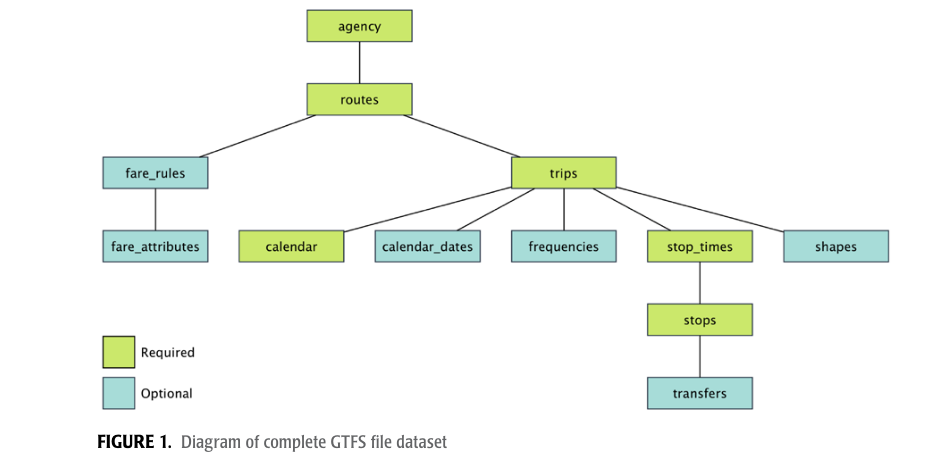
\includegraphics[width=0.85\textwidth]{Figures/Cap3/DiagramCompleteDataSetGTFS.png}
   \caption[Estructura relacional de archivos \gtfs{}]{Diagrama de la estructura
   relacional de los archivos que componen el estándar \gtfs{}.}
   \label{fig:gtfs-estructura}
   \fuentefigura{\citet{fortin2016innovative}, p.~21.}
 \end{figure}

El principio de comparación cuantitativa de redes que articula esta subsección
es el núcleo metodológico del Objetivo Específico 5 (§
\ref{subsec:obj-especificos}): calcular los indicadores $DI$, $T$ y $B(v)$ sobre
la red actual y sobre la red ampliada con el corredor anillar, y comparar los
resultados, es el procedimiento de planeación estratégica aquí descrito aplicado
al caso de la \zmvm{}. La demostración analítica del impacto hipotético del
Anillo Periférico no es un ejercicio especulativo, sino la aplicación directa de
esta metodología.
